% !TEX encoding = UTF-8 Unicode
%!TEX root = ../Main/thesis.tex
% !TEX spellcheck = en-US
%%=========================================
\documentclass[../Main/thesis.tex]{subfiles}
\begin{document}
\chapter[Fourier analysis and its application to bearing fault detection]{Fourier analysis and its application to bearing fault detection}
\label{sec:chapter2}

\section{An overview of Fourier analysis}
From solving differential equations to analyzing sound wave, images and signal in general, Fourier analysis has a profound impact in science and engineering. It provides a convenient way to transforming signals into sums of frequencies called frequency spectrum, and reveals unseen aspect of data. The bulk of Fourier analysis is to decompose a signal or more generally a function, into trigonometric extensions. 
\justify
 A signal can be viewed as a series of observations generated by a given process and recorded at discrete or continuous time interval. The underlying process might be the sum of given subprocesses. In this case, the frequency spectrum will reveal all the subprocesses characteristics.
This is illustrated in Figure \ref{fig:fft_domain}, where a signal (in dark) is decomposed into sinusoidal components (in blue). The sinusoidal components can be represented in a coordinate system with frequencies on the x axe and amplitudes on the y axe (in red). This is called the frequency domain. From the frequency domain we can observe a hight amplitude low frequency component. As we move toward high frequencies, the amplitudes decrease.
\begin{figure}[H] %  figure placement: here, top, bottom, or page
   \centering
   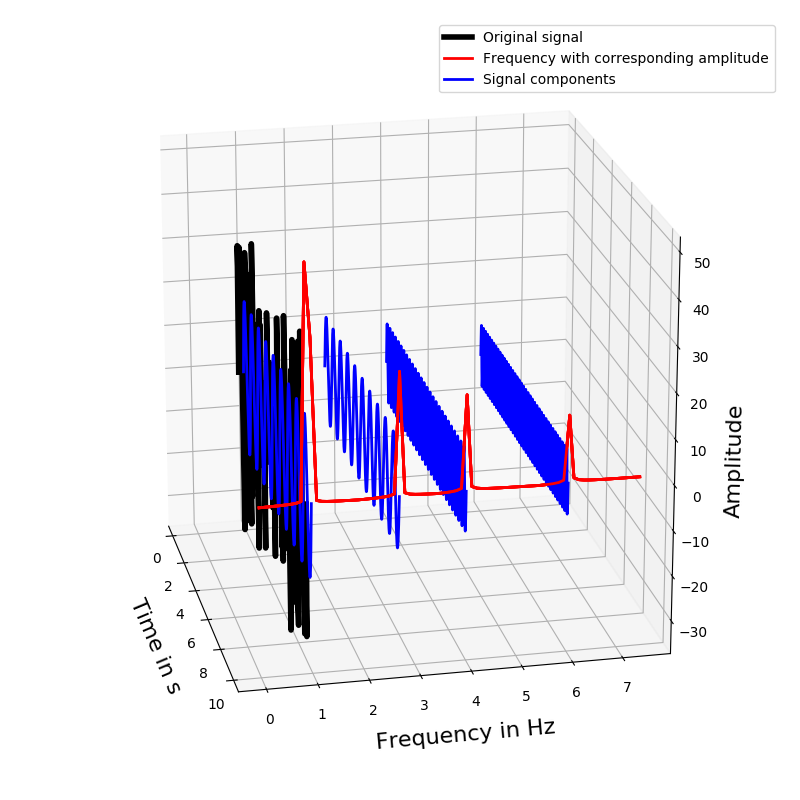
\includegraphics[width=6in]{../fig/fft_domain} 
   %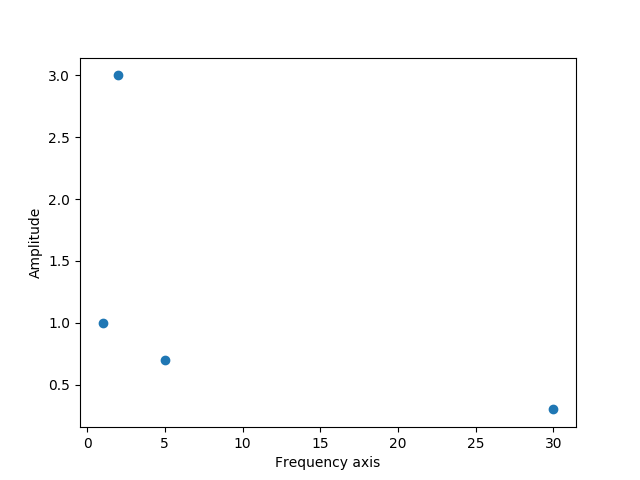
\includegraphics[width=2.5in]{freq} 
   \caption{}
   \label{fig:fft_domain}
\end{figure}
\justify
Fourier analysis is concerned with the general problem of periodic and non periodic functions approximation. The former and the latter are treated by Fourier series and Fourier transform, respectively. %Given a periodic function, its Fourier series is given as a discrete superposition of exponential functions, and its Fourier transform is given by continuous superposition of exponential functions.
%\justify
%Fourier analysis is used in a wide range of application, including signal processing, data compression, image analysis. The main objective is to take a signal or more generally a function, and decompose its in trigonometric functions. 
%%%%%%%%%%%%%%%%%%%%%%%%%%%%%%%%%%%%%%%%%%%%%%%%%%%%%%%%%%%%%

\subsection{Fourier series}
As previously mention, Fourier series is concerned with the general problem of periodic functions approximation. The basic ingredients required to approximate a function in this scenario are: a vector space, a basis, which is a subspace of the vector space, and a mathematical operation such as an inner product that maps two vectors to a real number. If a vector space has an inner product, we say that the vector space is an inner product space. 
\justify
Before continuing, we see the need to clarify some abbreviations. We use the letters $f$, $V$, $V_{0}$ for an arbitrary function, a vector space, and a subspace of a vector space, respectively.
Basis functions will be denoted by $\{  \varphi_{0}, \cdots,\varphi_{n}\}$, where $n$ can either be a finite integer or infinite. Having made this clarification, let explain the concept of function approximation. 
\justify
The function approximation process in light of Fourier series goes like this: Given an arbitrary function $f$ that we seek to approximate, we pick an appropriate vector space which we call $V$, such that $f\in V$. We define a subspace $V_{0}$ of the vector space $V$ and construct an inner product on $V_{0}$, if it does not exist. Furthermore, we fine an appropriate basis of $V_{0}$.  A basis of $V_{0}$ is a set of linearly independent vectors   $\{  \varphi_{0}, \cdots,\varphi_{n}\}$ in $V_{0}$, that span $V_{0}$. 
\justify
This means that any vector in $V_{0}$ can be written as a linear combination of the basis vectors. Once we have all this in place, the best approximation of the function $f$ is its orthogonal projection in the inner product space $V_{0}$. Figure \ref{figure:il} shows an illustration of a generic mechanism of function approximation by orthogonal projection, where $f_{0}$ is the orthogonal projection of $f$ in the subspace $V_{0}$ of $V$.
\justify
\begin{figure}[H]
\begin{center}
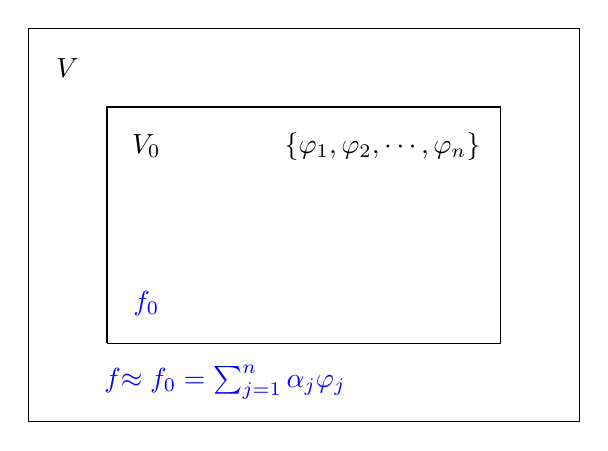
\begin{tikzpicture}
\path (0,0) coordinate (origin1);
\path(0.5,4.5) node (V){$V$};
\path(2.5,0.5) node (f){$\textcolor{blue}{f}\textcolor{blue} {\approx f_{0} = \sum_{j=1}^{n} \alpha_{j} \varphi_{j}}$};
\path (0,5) coordinate (topleft1);
\path (7,5) coordinate (topright1);
\path (7,0) coordinate (bottom1);
% draw
\draw (origin1) -- (bottom1) -- (topright1) -- (topleft1) -- (origin1);

% reactagle 2
\path (1,1) coordinate (origin2);
\path(1.5,3.5) node (V0){$V_{0}$};
\path(1.5,1.5) node (f0){$\textcolor{blue}{f_{0}}$};

\path (1,4) coordinate (topleft2);
\path (6,4) coordinate (topright2);
\path(4.5,3.5) node (b0){$ \{\varphi_{1}, \varphi_{2}, \cdots, \varphi_{n}\} $};
\path (6,1) coordinate (bottom2);
% draw
\draw (origin2) -- (bottom2) -- (topright2) -- (topleft2) -- (origin2);
\end{tikzpicture}
\end{center}
\caption{Illustration of a generic function approximation process of a function $f$ into a subspace $V_{0}$ of a vector space $V$. $\varphi_{j}$ are the basis functions and $\alpha_{j}$ are real numbers for $j=1,\cdots,n$.}
\label{figure:il}
\end{figure}

\justify
Having the generic function approximation defined in Figure \ref{figure:il} as a blue print, the Fourier space $V_{0}$ is a subspace of the space of all continuous functions of the interval $[0, T]$ and denoted by $C[0,T] $ which is $V$ in Figure \ref{figure:il}. The subspace $V_{0}$ of $V$ is spanned by 
\begin{equation}
\left\{1, \cos\left( \frac{2\pi t}{T} \right), \cdots,\cos\left( \frac{2\pi Nt}{T} \right), \sin\left( \frac{2\pi t}{T} \right), \cdots,\sin\left( \frac{2\pi Nt}{T} \right)   \right\}. \nonumber
\end{equation}
which corresponds to
\begin{equation}
\{\varphi_{1}, \varphi_{2}, \cdots, \varphi_{n}\}, \nonumber
\end{equation}
from figure \ref{figure:il}. Let $f$ be an arbitrary periodic function of period $T=2L$, defined on an interval of length $L$. Its Fourier series representation is then given by
\begin{equation}\label{eq:fs}
f_{n}(t) = \frac{a_{0}}{2} +\sum_{n=1}^{n}\left( a_{n} \cos\left( \frac{n\pi t}{L}\right) + b_{n} \sin\left( \frac{n\pi t}{L}\right)  \right), \end{equation}
where the coefficients $a_{0}, a_{1}, \cdots, b_{1}, b_{2},\cdots$, corresponding to the $\alpha_{j}$ in Figure \ref{figure:il}, are given by 
\begin{equation}\label{eq:fsc}
\begin{split}
a_{m} &= \frac{1}{L}\int_{-L}^{L}f(t)\cos\left( \frac{m\pi t}{L}\right) \mathrm{d}t,\quad m=0,1,2,\cdots\\
b_{n} &= \frac{1}{L}\int_{-L}^{L}f(t)\sin\left( \frac{n\pi t}{L}\right) \mathrm{d}t,\quad n=1,2,\cdots
\end{split}
\end{equation}
\justify
There are various condition under which the Fourier series given in (\ref{eq:fs}) converges. One such condition is the Dirichlet condition and is given by the following theorem:

\begin{theorem}
Suppose that $f$ is periodic with period $T$, and the following conditions are satisfied:
\begin{enumerate}
\item $f$ has a finite set of discontinuity in each period
\item $f$ contains a finite set of maxima and minima in each period
\item $\int_{0}^{T}|f|\mathrm{d}t <\infty$
\end{enumerate}

Then we have that 
\begin{equation}
\lim_{n\rightarrow \infty} f_{n}(t) = f(t) ,\nonumber
\end{equation}
for all t, except at those points t where f in not continuous.
\end{theorem}
Equation (\ref{eq:fs}) can be compactly written as an complex exponential expansion of the form
\begin{equation}\label{eq:fse}
f(t) = \sum_{n=1}^{N} c_{n}e^{\frac{2\pi i n t}{T}},
\end{equation}
where $T = 2L$,  $i$ is the imaginary number and the coefficients $c_{n}$ are given by
\begin{equation}
c_{n} = \frac{1}{T}\int_{-L}^{L}e^{\frac{2\pi i n t}{T}}f(t)\mathrm{d}t
\end{equation}
%%%%%%%%%%%%%%%%%%%%%%%%%%%%%%%%%%%%%%%%%%%%%%%%%%%%%%%%%%%%%%%%%%%%%%%%%%%%%%%%%%%%%
%%%%%%%%%%%%%%%%%%%%%%%%%%%%%%%%%%%%%%%%%%%%%%%%%%%%%%%%%%%%%%%%%%%%%%%%%%%%%%%%%%%%%
%%%%%%%%%%%%%%%%%%%%%%%%%%%%%%%%%%%%%%%%%%%%%%%
\subsection{Fourier transform and the fast Fourier transform}
On an application point of view, the Fourier series is limited. Let explain why. Most signal found in real application are non periodic waveform that vibrate at non integer frequencies. However, the Fourier series only deals with periodic functions. Its decomposes signals into trigonometric extensions in $[-\pi, \pi]$, that vibrates at integer frequencies. To circumvent the short coming of the Fourier series, the Fourier transform is introduced. Its decomposes non periodic functions into sinusoidal extensions that vibrates at frequencies that are real number on infinite time interval [ref]. This is of great practical importance, at least for bearing fault detection, since failure frequencies are often real numbers.
\justify
The Fourier transform $\hat{f}(s)$ of a given function $f$, is a complex valued function defined by the integral
\begin{equation}\label{eq:ft}
   \hat{f}(s) = \int_{-\infty}^{\infty}e^{-2\pi i s}f(t)\mathrm{d}t,
\end{equation}
assuming that $f$ is defined for all real numbers $t$ and $s\in\mathbb{R}$. The Fourier transform defined by (\ref{eq:ft}) gives a continuous spectrum of frequencies as opposed to the Fourier series of a periodic function which generates a discrete spectrum of frequencies. The function $f$ can be recover from the continuous spectrum of frequencies by taking the inverse Fourier transform to obtain
\begin{equation}\label{eq:ift}
f(t) = \int_{-\infty}^{\infty}e^{2\pi i s}\hat{f}(s)\mathrm{d}s,
\end{equation}
In technical semantics, we say that the Fourier transform $\hat{f}(s)$ is defined on the frequency domain, while $f(t)$ is defined on the time domain. This define a time and frequency duality. For any real number $s$, the square magnitude $|\hat{f}(s)|^{2}$ is called the power spectrum or the spectral power density. Its gives the energy of a signal in terms of frequency. The frequency domain and the time domain are related by the so called Parcevals identity
given by 
\begin{equation}\label{eq:parceval}
\underbrace{\int_{-\infty}^{\infty}|f(t)|^{2}\mathrm{d}t}_{\text{energy of the signal f}} = \underbrace{\int_{-\infty}^{\infty}|\hat{f}(s)|^{2}\mathrm{d}s}_{\text{Energy spectrum}}
\end{equation}
Equation (\ref{eq:parceval}) says that the total energy in the time domain is equal to the total energy in the frequency domain. The left hand side of Equation (\ref{eq:parceval}) defines the total energy of the signal $f$ while the right hand side gives what is called the energy spectrum, which is the total energy in the frequency domain. The latter quantifies the energy contribution of all frequencies.
\justify
The time and frequency duality defined above, allows time domain information to be recover in the frequency domain. To illustrate this fact, let assume that a vibration sensor records the vibrating movement of a bearing over a period of time. This measurement can be view as a function of time and reside in the time domain. By applying the Fourier transform, we can decompose the signal into frequencies which reside in the frequency domain. Assume further that the goal is to detect any failure incur by the bearing. For a bearing, the failure frequency can be computed based on the bearing geometrical characteristics. Once we known the failure frequency, it remains to search for it in the frequency domain. In the subsequent section we will discus how Fourier transform can be use to detect specific bearing failure frequencies.
For the time being, let discuss the conditions under which the integrals defined in equations (\ref{eq:ft}, \ref{eq:ift}) exist.
\begin{theorem}
If $f$ is a continuously differentiable function with 
\begin{equation}\label{eq:sumable}
\int_{-\infty}^{\infty}|f(t)|\mathrm{dt} <\infty,
\end{equation}
then
\begin{equation}
f(t) = \int_{-\infty}^{\infty}e^{2\pi i s}\hat{f}(s)\mathrm{ds}, \nonumber
\end{equation}
where $\hat{f}(s)$ the Fourier transform is given by
\begin{equation}
 \hat{f}(s) = \int_{-\infty}^{\infty}e^{-2\pi i s}f(t)\mathrm{dt}. \nonumber
\end{equation}
\end{theorem}
Thus if $f$ is continuously differentiable and the integral defined by (\ref{eq:sumable}) is absolutely convergent, the Fourier transform of $f$ exists. In cases where the latter condition is not satisfied, the Fourier transform still exists if the integral defined by (\ref{eq:sumable}) is conditionally convergent.
\justify
So far, in our discussion of Fourier transform, only continuous function (signal) have been mention. However, in many applications such as signal analysis, we are primarily dealing with discrete signals. Recall that a discrete signal has values at discrete times. For such signals, we need to apply the discrete Fourier transform.
\begin{definition}
Let $x = \{ x_{j} \}_{j = 0}^{n}$ 
be a sequence of real numbers. The discrete Fourier transform of $x$ denoted by $\hat{x}$ is the sequence
$\hat{x} = \{ \hat{x}_{k} \}$, where 
\begin{equation}
\hat{x}_{k} = \sum_{j=0}^{n-1}x_{j}\overline{w}^{jk} \text{with} \quad w = \exp\left(  \frac{2\pi i}{n} \right),\nonumber
\end{equation}
where $i$ is the imaginary complex number, $n$ is an integer and $\overline{w}$ denote the complex conjugate of $w$.
\end{definition}
Practically, the computation of the Discrete Fourier transform reduces to the following matrix computation
\begin{equation}\label{eq:mft}
\underbrace{
 \begin{pmatrix}
  \hat{x}_{0} \\
  \hat{x}_{1}  \\
  \hat{x}_{2}  \\
  \vdots  \\
  \hat{x}_{n-1}
 \end{pmatrix} 
 }_{\hat{x}}
 = 
 \underbrace{
 \begin{pmatrix}
  1 & 1 &1& \cdots & 1 \\
  1 & w & w^{2}&  \cdots & w^{n-1} \\
  1 & w^{2} & w^{4}&  \cdots & w^{2(n-1)} \\
  \vdots  & \vdots  & \vdots & \vdots&\vdots  \\
  1 & w^{n-1} & w^{2(n-1)}&  \cdots & w^{(n-1)^{2}} \\
 \end{pmatrix}
 }_{F_{n}}
 \underbrace{
 \begin{pmatrix}
  x_{0} \\
  x_{1}  \\
  x_{2}  \\
  \vdots  \\
  x_{n-1}
 \end{pmatrix}
 }_{x},
\end{equation}
where $F_{n}$ is a symmetric matrix. The matrix operation defined in equation (\ref{eq:mft}) requires $n^{2}$ multiplications. For large $n$, this can incur a significant overhead. Fortunately, since the matrix $F_{n}$ is symmetric, the number of multiplications can be reduced to $5n\log_{2}(n)$, by applying the so called fast Fourier transform algorithm. 
\begin{equation}
\hat{x} = \sum_{j = 0}^{\frac{n}{2}-1}\overline{W}^{jk} + \overline{w}^{k}\left(   \sum_{j=0}^{\frac{n}{2}-1}x_{2j+1}\overline{W}^{jk}\right)
\end{equation}
 
%%%%%%%%%%%%%%%%%%%%%%%%%%%%%%%%%%%%%%%%%%%%%%%%%%%%%%%%%%%%%%%%%%%%%%%%%%%%%%%%%%%%%
%%%%%%%%%%%%%%%%%%%%%%%%%%%%%%%%%%%%%%%%%%%%%%%%%%%%%%%%%%%%%%%%%%%%%%%%%%%%%%%%%%%%%

\section{Application of Fourier transform for bearing fault detection: a case study}
In this section we present a case study where Fourier analysis is used to detect various bearings failure frequencies. We start by describing the experimental setup for the case study, followed by the methodology for fault detection
\subsection{Description of the case study}
The data used in this case study was generated by the Intelligence Maintenance System (IMS) [link]. Three separate experiments involving four bearings were performed on a motor. In each experiment, a one second vibration signal snapshot was recorded every five or ten minutes [reference]. Each vibration signal or what we could call sample, consists of 20 480 data points with a sampling rate of 20 000 Hz.
\justify
The sampling rate also called sampling frequency, is the average number of sample points obtained per second during the sampling process. The sampling process is the reduction of an analog signal to a digital signal. The analog signal is the continuous time signal, while the digital signal is the discrete time signal of interest.
\begin{figure}[H] %  figure placement: here, top, bottom, or page
   \centering
   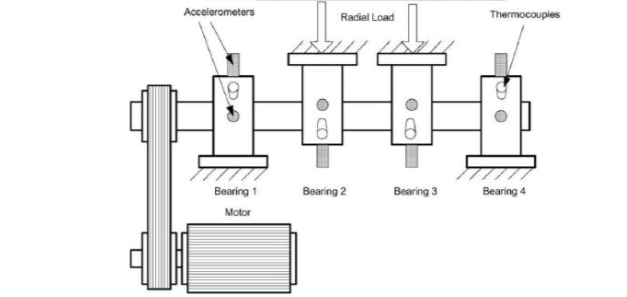
\includegraphics[width=8in]{../fig/experiment} 
   \caption{Experimental set up. [reference]}
   \label{fig:exp}
\end{figure}
\justify
Figure \ref{fig:exp} shows the experimental setup. Four bearings support a rotating shaft, driven by an AC motor through rub belts. The motor rotates at 2000 rotations per minute, while the bearings are subjected to a constant radial force of 6000 lbs [ref]. In the first experiment, eight accelerometers were used, two on each bearing. One for the radial position and the other for the axial position. In the second and third experiment, four accelerometers were used, one for each bearing.
An accelerometers is a sensor that measures vibration signals, in particular the acceleration experience by a bearing. Axial signal are the signal measured by the accelerometers along the axis of the motor shaft, while radial signal are measure along the perpendicular direction of the motor shaft.
\justify
At the end of the first experiment, inner race defect occurred in bearing number 3 and roller element defect occurred in bearing number 4. At the of the second and third experiment, outer race defect occurred in bearing number 1 and number 3, respectively. In the next section we define the different types of bearing faults such as inner race defect, outer race defect and roller element defect. 

%%%%%%%%%%%%%%%%%%%%%%%%%%%%%%%%%%%%%%%%%%%%%%%%%%%%%%%%%%%%%%%%%%%%%%%%%%%%%%%%%%%%%
%%%%%%%%%%%%%%%%%%%%%%%%%%%%%%%%%%%%%%%%%%%%%%%%%%%%%%%%%%%%%%%%%%%%%%%%%%%%%%%%%%%%%


\subsection{Bearing faults}
As pointed out earlier, the bearing failure frequencies depends on the geometry of the bearing and the rotating speed of the motor. Figure \ref{fig:bearing} shows a blow up view of a bearing. In the figure we see the outer ring of the bearing (1), the cage (3) which holds the cylindrical rolling elements (2) and the inner race (4 and 5).
\begin{figure}[H] %  figure placement: here, top, bottom, or page
   \centering
   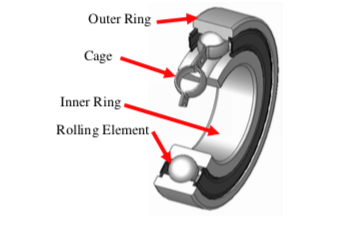
\includegraphics[width=3.2in]{../fig/bearing} 
    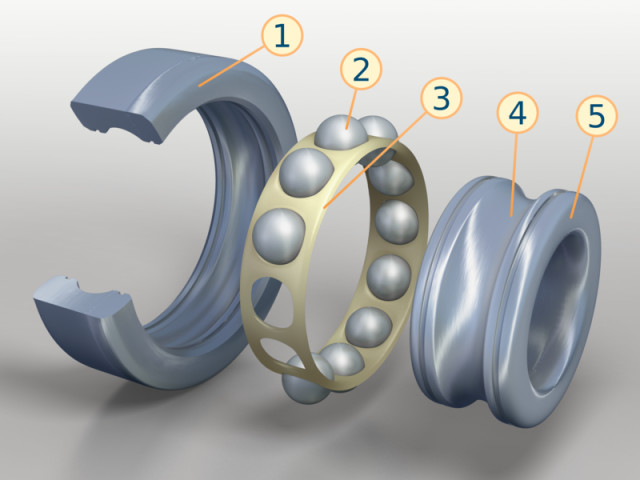
\includegraphics[width=3.2in]{../fig/bearing-s} 
   \caption{Geometrical description of a bearing left(ref), right(ref)}
   \label{fig:bearing}
\end{figure}
\justify
Inner race defect and outer race defect are defect occurring at the inner race and outer race, while roller element defect also called ball spin happens when a roller element is defectuous. Any of the defect occurs at a specific frequency that can be computed based on the bearing geometry and the rotation speed of the machine. inner race defect occurs at a frequency called ball pass frequency inner race (BPFI), outer race defect occurs at a frequency call ball pass outer frequency outer race (BPFO) and roller element defect occurs at a frequency call ball spin frequency (BSF). They are expressed in Hz in terms of the bearing geometry as 
\begin{equation}\label{eq:bpfi}
BPFI = \frac{nb}{2}S\left( 1 +  \frac{BD}{PD}\cos(\beta)  \right)
\end{equation}

\begin{equation}\label{eq:bpfo}
BPFO = \frac{nb}{2}S\left( 1 -  \frac{BD}{PD}\cos(\beta)  \right)
\end{equation}

\begin{equation}\label{eq:bpfi}
BSF = \frac{PD}{2BD}S\left( 1 -  \left(\frac{BD}{PD}\cos(\beta)\right)^{2}  \right)
\end{equation}
\clearpage
where 
\begin{itemize}
\item S is the rotating speed of the motor
\item nb is the number of cylindrical balls (roller elements)
\item BP is the the ball diameter
\item PD is the pitch diameter
\item $\beta$ is the contact angle
\end{itemize}
The pitch diameter is the perpendicular distance from the center of one ball to the center of the ball located at the end. The contact angle can be taken to be zero?
%%%%%%%%%%%%%%%%%%%%%%%%%%%%%%%%%%%%%%%%%%%%%%%%%%%%%%%%%%%%%%%%%%%%%%%%%%%%%%%%%%%%%
%%%%%%%%%%%%%%%%%%%%%%%%%%%%%%%%%%%%%%%%%%%%%%%%%%%%%%%%%%%%%%%%%%%%%%%%%%%%%%%%%%%%%


\subsection{Failure detection methodology}
Given a vibration signal measured from an accelerometer, our intent is to detect the presence of a forcing frequency. By forcing frequency we refer to either BPFO, BPFI or BSF. Recall that a forcing frequency is a fancy name for failure frequency. We will refer to the vibration signal as the time domain signal, as it is customary to do so. Since the forcing frequencies are in Hz, the time domain signal must be transformed into frequency domain signal. The frequency domain signal is also called the frequency spectrum. The reader can refer to Figure \ref{fig:fft_domain} for a reminder. Once we have the frequency spectrum corresponding to the original time signal, we can look for the presence of any forcing frequency.
\justify
There are four steps in transforming time domain signal into frequency domain signal: A band pass filtering, enveloping, a low pass filtering and a fast Fourier transformation.
Figure \ref{fig:fft-process} shows a schematic description of the entire process. Let elaborate on it.  A vibration signal from a bearing accelerometer contains not only the vibration signal of the bearing, but also the signal from other components, such as motor, shaft and so on.
\justify
The band pass filter allows signal within a given band of frequency to seep through, while attenuating all other signal. The band of allowed frequencies is bounded bellow and above by two parameters: The low cut-off frequency and the high cut-off frequency, respectively.
%The intent is to only capture bearing vibration signal and ignore any other. Once this done, the demodulation extract the high frequency time domain signal and a low pass filter extract the low frequency. The Fast Fourier transform is then applied to the time domain signal to generate the frequency spectrum.
\begin{figure}[H]
\begin{tikzpicture}
  [node distance=.8cm,
  start chain=going below,]
     \node[punktchain, join] (intro) {Signal};
     \node[punktchain, join] (probf)      {Band pass filtering};
     \node[punktchain, join] (investeringer)      {Enveloping};
     \node[punktchain, join] (perfekt) {Low pass filtering};
     \node[punktchain, join, ] (emperi) {Fast Fourier transform};
     % \node (asym) [punktchain ]  {Asymmetrisk information};
      \begin{scope}[start branch=venstre,
        %We need to redefine the join-style to have the -> turn out right
        every join/.style={->, thick, shorten <=1pt}, ]
        \node[punktchain, on chain=going left, join=by {->}] (risiko) {Frequency spectrum and amplitude};
      \end{scope}
      \begin{scope}[start branch=hoejre,]
      %\node (finans) [punktchain, on chain=going right] {Det finansielle system};
    \end{scope}
    \end{tikzpicture}
  \caption{Process of obtaining a frequency spectrum from an input signal}
   \label{fig:fft-process}
\end{figure}
\justify
The enveloping step corresponds to rectifying the signal by accounting only for the positive part of the signal. Let $E(t)$ be the signal resulting from the enveloping process. Let $x(t)$ is the time domain signal, and let its Hilbert transform be denoted by $H(t)$. Then we have
\begin{equation}
H(t) = \frac{1}{\pi}P\int_{-\infty}^{+\infty}\frac{x(t)}{t-\tau}\mathrm{d}\tau
\end{equation}
\begin{equation}
E(t) = \sqrt{H(t)^{2}+ x(t)^{2}}
\end{equation}
where $P$ is the Cauchy principal value. After the enveloping process, the resulting signal is filtered by removing hight frequency noise and the fast Fourier transform is applied to obtain the frequency spectrum.
\justify
Once we have found the frequency spectrum and the corresponding amplitude, we search any of the forcing frequency and record their amplitude in time. Base on a predefine limit, an alarm is raised when the amplitude is above the limit.

%%%%%%%%%%%%%%%%%%%%%%%%%%%%%%%%%%%%%%%%%%%%%%%%%%%%%%%%%%%%%%%%%%%%%%%%%%%%%%%%%%%%%
%%%%%%%%%%%%%%%%%%%%%%%%%%%%%%%%%%%%%%%%%%%%%%%%%%%%%%%%%%%%%%%%%%%%%%%%%%%%%%%%%%%%%


\clearpage
\subsection{Failure detection results}
In this section we present the results from applying Fourier analysis to detecting one type of fault in bearing, namely: ball pass frequency outer race defect (BPFO). The methodology can easily be extended to other forcing frequencies as well, but we limit ourselves to BPFO to avoid any redundancy. Recall that BPFO occurs when a defect is initiated in the outer ring of the bearing. The reader can refer to Figure \ref{fig:bearing} for a detailed geometrical description of a bearing. The experimental setup for the bearings are given in Figure \ref{fig:exp}. The bearing type used in this experiment are manufactured by the company Rexnord, and are of type Rexnord ZA 2115, with BPFO forcing frequency  given by 
\begin{equation}
BPFO = 236.4 Hz, %\quad BPFI = 296.8 Hz \nonumber
\end{equation}

%%%%%%%%%%%%%%%%%%%%%%%%%%%%%%%%%%%%%%%%%%%%%%%%%%%%%%%%%%%%%%%%%%%%%%%%%%%%%%%%%%%%%
%%%%%%%%%%%%%%%%%%%%%%%%%%%%%%%%%%%%%%%%%%%%%%%%%%%%%%%%%%%%%%%%%%%%%%%%%%%%%%%%%%%%%


\subsubsection{Forcing frequency detection}
We apply the process described in Figure \ref{fig:fft-process} to experiment number 2.
In the latter, successive vibration samples where obtained from four bearings: Bearing number 1,2,3 and 4, resulting in 984 samples for each bearing.  
The samples were obtained by installing accelerometers on each bearing. Recall that an accelerometer in this context, is a sensor that measures the acceleration experienced by a bearing.
The experiment started in February 12, 2004 at 10:32:39 and ended in February 19, 2004 at 06:22:39, and vibration samples were obtained every ten minutes [ref].
At the end of the experiment, BPFO defect occurs in bearing number 1 [ref]. Figure \ref{fig:bearing1-experiment2} shows the vibration signal from sample obtained in  February 18, 2004, at 16:32:39, from bearing number 1. Figure \ref{fig:bearing1-experiment2-fft} shows the corresponding frequency spectrum obtained by applying the process described in Figure \ref{fig:fft-process}.
\justify
In the frequency spectrum, we can clearly identify the BPFO frequency (in orange), which has the largest amplitude in the spectrum. We can also observe three harmonics of the BPFO. BPFO harmonics are multiple frequency of the BPFO frequency. Here we observe $2\times$BPFO and $3\times$BPFO harmonics. One of the salient features of the BPFO frequency is the presence of harmonics [ref:Vib analy training manuel cat1]. 
\begin{figure}[H] %  figure placement: here, top, bottom, or page
   \centering
   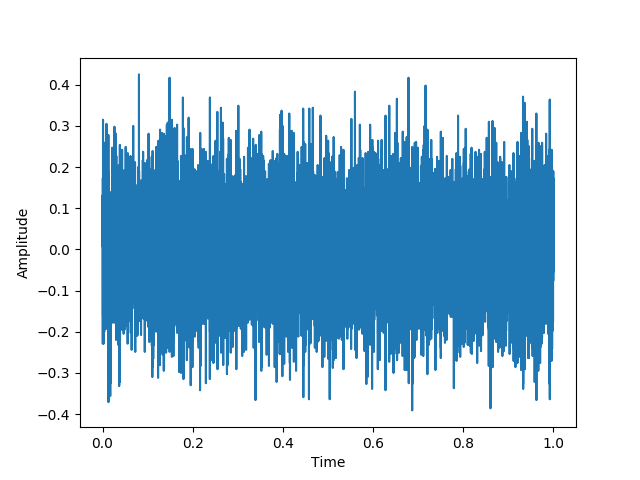
\includegraphics[width=4.9in]{../fig/experiment2_bearing1.png} 
   \caption{Vibration signal obtained in February 18, 2004, at 16:32:39, from bearing number 1 in  experiment number 2.}
   \label{fig:bearing1-experiment2}
\end{figure}
%%%%%%%%%%%%%
\begin{figure}[H] 
   \centering
   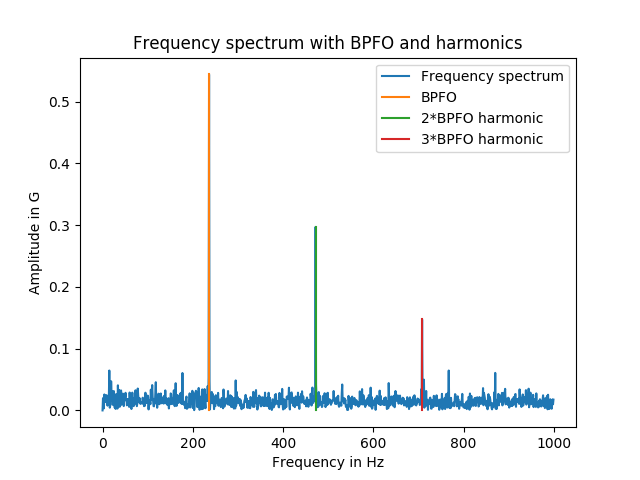
\includegraphics[width=4.9in]{../fig/experiment2_bearing1_fft.png} 
   \caption{Frequency spectrum obtained from the vibration signal obtained in February 18, 2004, at 16:32:39, of bearing number 1,  in  experiment number 2.}
   \label{fig:bearing1-experiment2-fft}
\end{figure}
\justify
In contrast to Figure \ref{fig:bearing1-experiment2-fft}, Figure \ref{fig:bearing2-experiment2-fft}, \ref{fig:bearing3-experiment2-fft} and \ref{fig:bearing4-experiment2-fft}, show  the frequency spectrum of bearing number 2,3 and 4, respectively. The frequencies spectrum were obtained in February 18, 2004, at 16:32:39 as well. No apparent large peak can be observe in these spectrum. This correlates with the fact that the spectrum are from bearings with no defect. 
\begin{figure}[H] 
   \centering
   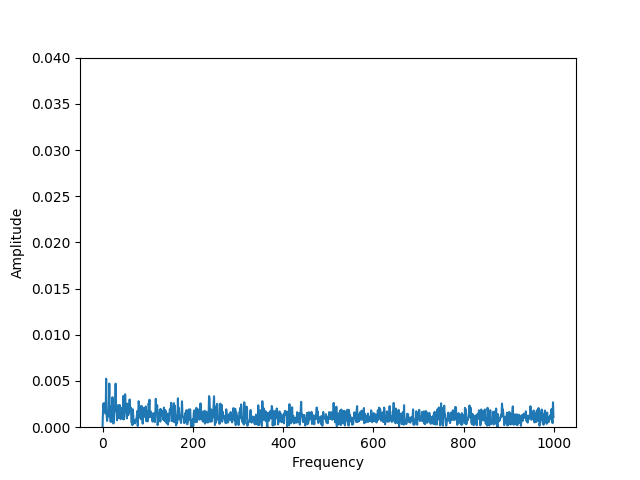
\includegraphics[width=4.9in]{../fig/experiment2_bearing2_fft.png} 
   \caption{Frequency spectrum obtained from vibration signal obtained in February 18, 2004, at 16:32:39, of bearing number 2, in experiment 2.}
   \label{fig:bearing2-experiment2-fft}
\end{figure}

\begin{figure}[H] 
   \centering
   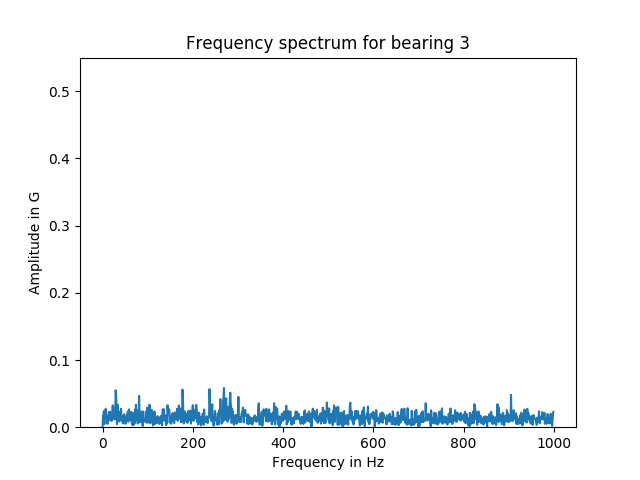
\includegraphics[width=4.9in]{../fig/experiment2_bearing3_fft.png} 
   \caption{Frequency spectrum obtained from vibration signal obtained in February 18, 2004, at 16:32:39, of bearing number 3, in experiment 2.}
   \label{fig:bearing3-experiment2-fft}
\end{figure}

\begin{figure}[H] 
   \centering
   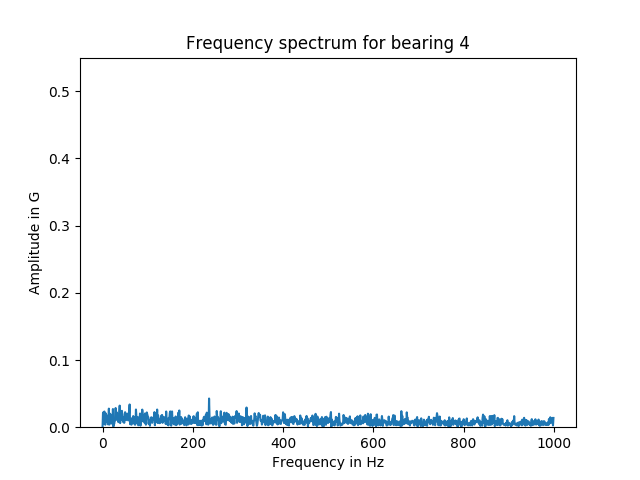
\includegraphics[width=4.9in]{../fig/experiment2_bearing4_fft.png} 
   \caption{Frequency spectrum obtained from vibration signal obtained in February 18, 2004, at 16:32:39, of bearing number 4, in experiment 2.}
   \label{fig:bearing4-experiment2-fft}
\end{figure}
\justify
To show the potential propagation of faults in the bearing, the amplitude corresponding to the BPFO forcing frequency are recorded for all four barings, for the duration of the experiment. Figure \ref{fig:experiment2_bearing_fft_amp}  shows the BPFO amplitude for each sample. At the beginning of the experiment, all bearing have a very low BPFO amplitude. However, after four days, the onset of failure is initiated in bearing number 1 and the amplitude of the forcing frequency keeps increasing.
% trend as the experiment evolves. We can observe that at the beginning of the experiment, all bearing have a very low BPFO amplitude. However, at [date], the BPFO amplitude of bearing number 1 starts increasing. As the experiment evolves, the amplitude increases almost steadily, until failure occurs. In contrast to bearing 1, bearing 2, 3 and 4, the BPFO amplitude are relatively steady during the experiment, and only a slight increase is noticeable at the end of the experiment.
\begin{figure}[H] 
   \centering
    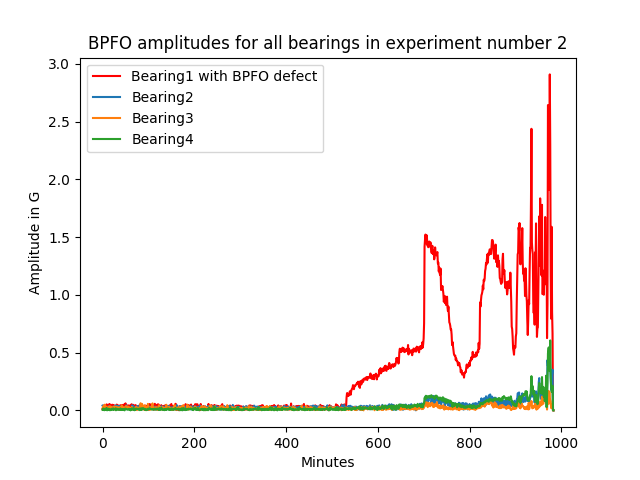
\includegraphics[width=4.9in]{../fig/experiment2_bearing_fft_amp.png}
  % 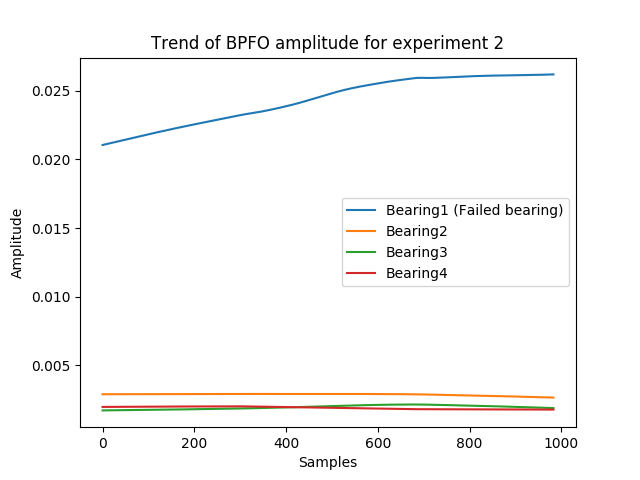
\includegraphics[width=4.4in]{../fig/experiment2_bearing_fft_trend.png} 
   \caption{BPFO amplitude evolution for all bearings over time}
   \label{fig:experiment2_bearing_fft_amp}
\end{figure}
\justify
This increase is captured by Figure \ref{fig:experiment2_bearing_fft_trend}, which displays the trend component of Figure  \ref{fig:experiment2_bearing_fft_amp}.
The trend components are extracted by using the seasonal trend decomposition method based on LOESS (STL) [ref]. The method consists in sequentially applying the LOESS smoother (Locally Estimated Scatter Smoother) to the data [ref]. The STL will be extensively used in this work for trend and seasonal estimation and will be explained in detail in chapter 3. For the time being, let just say that the STL provides a robust seasonal trend estimation method and deals very well with missing or erroneous data points [ref]. In addition, it can be apply with ease to long time series, due to its computational efficient feature [ref].
\justify
Having computed the trends from Figure  \ref{fig:experiment2_bearing_fft_trend}, We ask the following valid question: Is there a pattern in the trend?  We limit ourselves to bearing number 1. In an attempt to answer this question, we plot the derivative of the trend given in figure  \ref{fig:grad_trend}. The later shows three distinct phases, which matche the correlated structure of the trend given in Figure \ref{fig:experiment2_bearing_fft_trend}. 
\begin{figure}[H] 
   \centering
   % 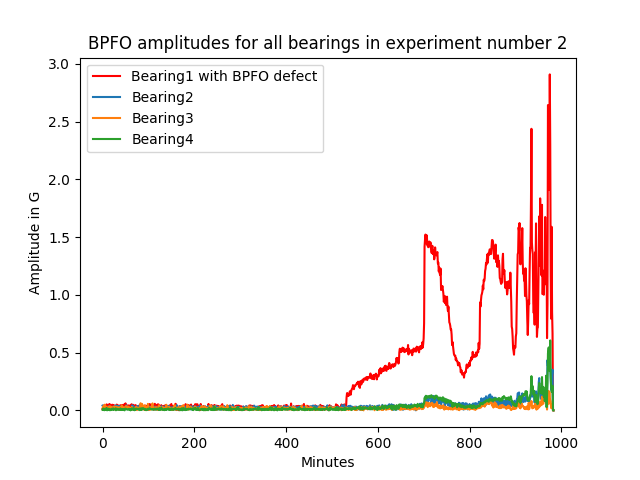
\includegraphics[width=4.4in]{../fig/experiment2_bearing_fft_amp.png}
   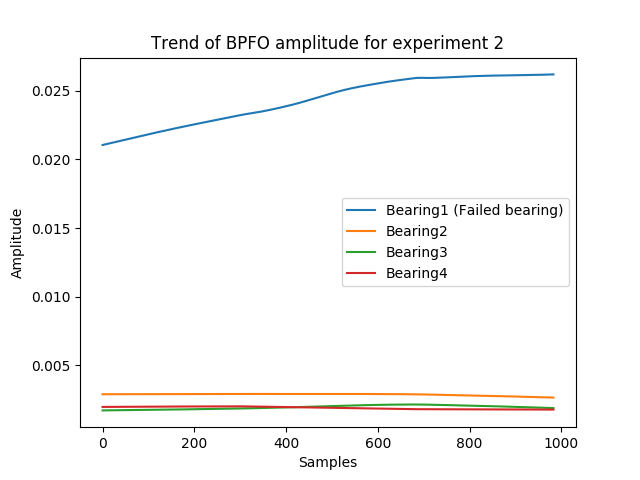
\includegraphics[width=4.9in]{../fig/experiment2_bearing_fft_trend.png} 
   \caption{Trend for BPFO for each bearing over time}
   \label{fig:experiment2_bearing_fft_trend}
\end{figure}
\begin{figure}[H] %  figure placement: here, top, bottom, or page
   \centering
   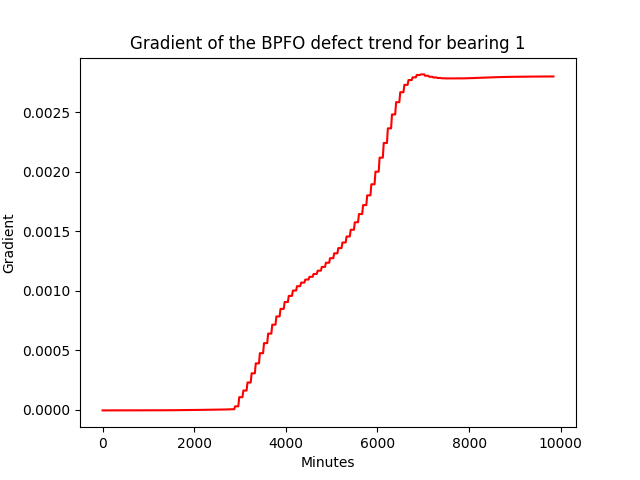
\includegraphics[width=4.9in]{../fig/bearing1_bpfo_trend_grad.png} 
   \caption{Gradient of the trend of BPFO forcing frequency amplitude for bearing 1}
   \label{fig:grad_trend}
\end{figure}
\clearpage
\justify
During the first phase, the derivative is constant, which implies that there is no change in the trend. This is followed by a rapid increase in the derivative. This phase is the onset and rapid propagation of failure within the bearing. In the last phase, the derivative is relatively constant. At this stage the bearing can fail at any given moment. A second and equally valid question is the following: Can we predict the failure time of the bearings? In an other word, can we estimate the remaining useful life of the bearings, based on the trend shown in Figure \ref{fig:experiment2_bearing_fft_trend}? In the next subsection we propose a methodology to tackle the latter question.
%%%%%%%%%%%%%%%%%%%%%%%%%%%%%%%%%%%%%%%%%%%%%%%%%%%%%%%%%%%%%%%%%%%%%%%%%%%%%%%%%%%%%
%%%%%%%%%%%%%%%%%%%%%%%%%%%%%%%%%%%%%%%%%%%%%%%%%%%%%%%%%%%%%%%%%%%%%%%%%%%%%%%%%%%%
\subsubsection{Trend based remaining useful life estimation}
In Figure  \ref{fig:experiment2_bearing_fft_trend}, we can observe the trend of bearing 1,2,3 and 4. The four bearings are of the same type and operate under the same condition. Since bearing number 1 failed, we used it as the reference bearing. The goal is to find the time at which the remaining working bearing will fail. We denote this time by $t_{f}$. To compute the latter, we assume that when the remaining bearing fail, the energy they produce will be approximately the same as the failed bearing. Let $E_{1}$ be the energy produced by bearing 1. This energy can be approximated by the area under the red curve in Figure \ref{fig:experiment2_bearing_fft_trend}. Furthermore, let $f_{i}$ be the BPFO amplitude trend define in Figure  \ref{fig:experiment2_bearing_fft_trend}, where $i$ denote bearing number $i= 1,2,3,4$. Then
\begin{equation}
\int_{0}^{t_{f}} f_{i}(t)\mathrm{dt}=E_{1} = \int_{0}^{t_{1}} f_{1}(t)\mathrm{dt}, \quad i = 2,3,4
\end{equation}
where $t_{1}$ is the time at which bearing 1 failed. We can estimate $f_{i}, i = 2,3,4$ by either a polynomial or an exponential function based on the shape of the trend in Figure \ref{fig:experiment2_bearing_fft_trend}.
For a $p$ order polynomial we get
\begin{equation}\label{eq:rul}
\int_{0}^{t_{f}} \theta_{0}+\theta_{1}t+\cdots \theta_{p}t^{p} \mathrm{dt}=E_{1} = \int_{0}^{t_{1}} f_{1}(t)\mathrm{dt}, \quad i = 2,3,4
\end{equation}
where $\theta_{j}, j = 0,\cdots,p$ is a constant. After integration, equation (\ref{eq:rul}) reduces to 
\begin{equation}\label{eq:rul1}
\theta_{0}t_{f}+\theta_{1}t_{f}^{2}+\cdots \theta_{p}t_{f}^{p+1} =E_{1} = \int_{0}^{t_{1}} f_{1}(t)\mathrm{dt}, \quad i = 2,3,4.
\end{equation}
It remains now to estimate the coefficients $\theta_{j}, j = 0,\cdots,p$, based on the available trend data in Figure \ref{fig:experiment2_bearing_fft_trend}. To do so, we let the objective function $\mathcal{O}(t_{f})$ be defined by 
\begin{equation}
\mathcal{O}(t_{f}) = \theta_{0}t_{f}+\theta_{1}t_{f}^{2}+\cdots \theta_{p}t_{f}^{p+1}-E_{1},
\end{equation}
and use the least square method to estimate the coefficients $\theta_{j}, j = 0,\cdots,p$
%After detecting the presence of a forcing frequency and recording the amplitudes, one can perform for example extrapolation, to predict the evolution of the amplitude. Looking at Figures  \ref{fig:experiment2_bearing_fft_amp}  and \ref{fig:experiment2_bearing_fft_trend}, we clearly see that extrapolating on the trend will be much easier than on the amplitude. The trend in Figure  \ref{fig:experiment2_bearing_fft_trend} is obtained from the robust seasonal trend estimation STL (Seasonal trend based on Loess) [ref].
%\justify
%The STL method is base on .....(Explain more about STL)

























\blankpage
\end{document}

